\documentclass[12pt,fleqn]{article}\usepackage{../common}
\begin{document}
Ders 4

Delta fonksiyonlari

Bugun su turdeki diferansiyel denklemlere bakacagiz

\[ -\frac{d^2u}{dx^2}=\delta(x-a) \]

\[ u(0) = 0, \ u(1) = 0 \]

Bu denklem $a$ noktasinda bir noktasal yuku temsil ediyor, delta denklemi
$\delta$ isareti ile gosteriliyor, delta kelimesi fizikte ve matematikte
genelde ``farklilik'' anlaminda kullanilir. Fonksiyonel anlamda $\delta$
sifir oldugu yerde sonsuzluk degeri verir, geri kalan her yerde sifir
degeri verir.

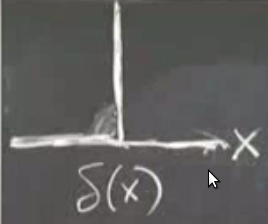
\includegraphics[height=2cm]{4_1.png}

Eger 0 yerine baska bir noktada agirlik koymak istiyorsak, $x-a$
kullanabiliriz, boylece $\delta(..)$'ya $a$ uzerinde sifir gider, ve o
nokta sonsuz degeri dondurur.

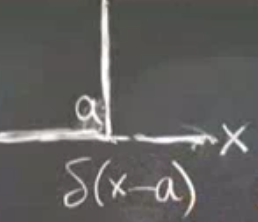
\includegraphics[height=2cm]{4_2.png} 

Not: Noktasal yuk fiziksel olarak olasiligi az bir olay olabilir. 

Delta fonksiyonlarinin bazi ozellikleri

\[ \int_{-\infty}^{\infty} \delta(x) dx = 1 \]

Yani delta fonksiyonunun tamaminin altinda kalan alan 1 degerine
esittir. Daha genel olarak dusunelim. Delta fonksiyonunu baska bir
fonksiyona ``karsi'' (onunla carparak) entegre edersem ne olur? 

\[ \int_{-\infty}^{\infty} \delta(x)g(x) dx = g(0)\]

Bu esitligin ispati dokumanin altinda.

Grafiksel olarak delta fonksiyonunu entegre edince sunu elde ederiz

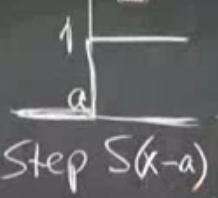
\includegraphics[height=2cm]{4_3.png}

Bu fonksiyona adim (step) fonksiyonu, ya da Heaviside fonksiyonu adi
veriliyor. 

Bir kez daha entegre edince

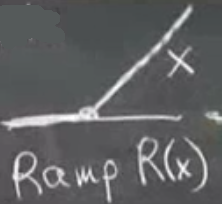
\includegraphics[height=2cm]{4_4.png}

Yokus (ramp) fonksiyonu elde ediyoruz. Bir kere daha entegre

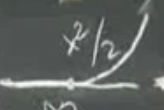
\includegraphics[height=2cm]{4_5.png}

Bir kere daha

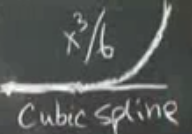
\includegraphics[height=2cm]{4_6.png}

Bu son fonksiyon kupsel spline fonksiyonudur, soyle ifade edilir:

\[ C = 
\left\{ \begin{array}{ll}
0 & x \le 0 \\
x^3 / 6 & x \ge 0
\end{array} \right.
 \]

Simdi tersten dusunelim, bir spline $C$'nin uc kere turevini alsak, sifir
noktasinda hangi deger geri gelir? $C'''(0) = 1$ degeridir, sifirdan once
ise sifirdir. Bu ilginctir, kupsel spline son derece puruzsuz (smooth) bir
fonksiyondur, fakat, tureve bakinca iyice anliyoruz ki, aslinda iki tane
farkli fonksiyondur. Kupsel spline'larin bu ozelligi CAD programlarinda,
cizimlerde cok ise yariyor.

Dort kere turevi alirsak yani $C''''$ nereye geliriz? $\delta$ fonksiyonuna
doneriz. 4. turev diferansiyel denklemlerde kullanilir, 4. turevin bir yuke
esitlinmesi cubuklarin (beam) bukulmesini modellerken kullanilir. Biyoloji,
mekanik konularinda cogu denklem 2. seviyedendir, 4. seviye nadirdir. 

Basa donersek: su denklemin genel cozumu nedir?

\[ -\frac{d^2u}{dx^2}=\delta(x-a) \]

Ilk once ozel (particular) cozumu bulalim. Ikinci turevinin negatifi delta
fonksiyonu olan fonksiyon nedir? Ustte ardi ardina entege ederken zaten bunu
irdelemistik, isareti degistiriyoruz tabii cunku simdi negatiflik var, ama
aradigimiz yokus fonksiyonu.

\[ u(x) = -R(x-a) \]

Isimiz bitti mi? Hayir. Ikinci t�revin s�f�ra e�it oldugu iki cozum daha
laz�m, iki homojen cozum yani, bunlardan biri $C$ digeri $Dx$. Cunku
elimizde tatmin edilmesi gereken iki tane s�n�r sart� var. 

\[ u(x) = -R(x-a) + C + Dx\]

Sinir sartlarini yerine koyalim

$x=0$ icin $0 = 0 + C + 0$. Rampa fonksiyonu $a$'dan yukselmeye baslayan,
egimi $x-a$ olan, baslangicta sifir olan bir fonksiyondur. 

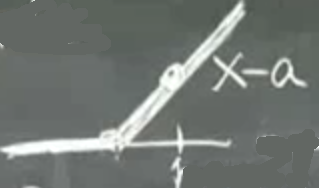
\includegraphics[height=2cm]{4_10.png}

$x=1$ noktasinda rampanin fonksiyonunun degeri $1-a$'dir. 

Yerine koyalim: $C = 0$. Onu kullanarak devam edelim, ikinci sart icin:

\[ u(x) = -R(x-a) + C + Dx \]

\[ -(x-a)+C+Dx = 0 \]

$C = 0$ ise

\[ -(1-a) + D = 0 \]

\[ D = 1-a \]

Tamami

\[ u(x) = -R(x-a) + (1-a)x \]

$a$ noktasi sonrasinda rampa fonksiyonu $x-a$ olduguna gore

\[ -(x-a) + (1-a)x = -x + a + x -ax = a - ax = a(1-x)\]

Grafik

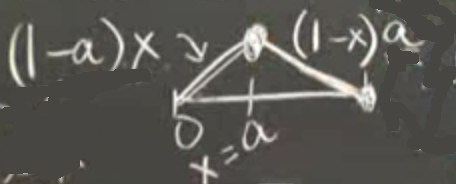
\includegraphics[height=2cm]{4_7.png}

$u(x)$'in kesintisiz (continuous) bir fonksiyon oldugunu
soyleyebiliriz. $u'(x)$ 1 kadar asagi iner. Egimi (slope) grafiklersek
nasil olur?

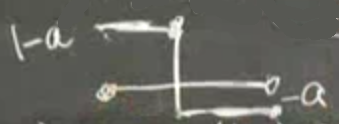
\includegraphics[height=2cm]{4_8.png}

Problemi fiziksel sekilde gorsellemek gerekirse, iki ucu sabitlenmis
elastic cubugu cizelim:

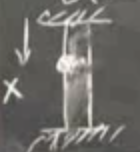
\includegraphics[height=2cm]{4_9.png}

Cubugun uzerindeki noktayi oraya asilmis bir agirlik olarak
dusunelim. $\delta(x-a)$ ile belirtmeye calistigimiz bu degil mi, bir
noktaya konsantre bir agirlik uyguluyoruz. Bu agirligi uygulayinca ne olur?
Nokta altinda s�k�sma, ustunde ise esneme olur. 

$u(x)$ tabii ki hep pozitiftir, yani cubugun tum noktalari asagi iner. Ama
bazi noktalar uzerinde s�k�sma, pozitif egim, digerleri uzerinde esneme
(negatif egim) vardir. 

Bir ucu serbest, digeri sabitlenmis problemi cozelim. 

\[ u'' = \delta(x-a) \]

\[ u'(0) = 0, \ u(1) = 0 \]

Sartlari kullaninca, 

\[ u(x) = - R(x-a) + Cx + D \]

$x=0$ noktasinda rampa daha baslamadi, $Cx + D$ kalir, turevi $C$, esittir
sifir. $C = 0$. $u(x)$ grafigi neye benzer?

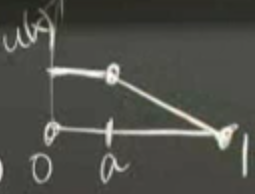
\includegraphics[height=2cm]{4_11.png}

Elastik cubuga ne olacak?

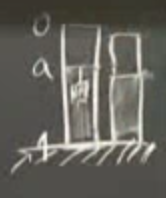
\includegraphics[height=2cm]{4_12.png}

Gri olarak nitelenen yer $a$'nin altinda olan yer, ve ol bolum bir s�k��ma
yasadi. Onun ustundeki bolum de tamamen asagi dogru indi, ama tum noktalari
ayni miktarda asagi indi, o bolgede $x$ degistikce ``degisim degismiyor'',
ki $u'$ turevinin tanimi bu degil mi? 

Soru: $u(x)$'in y eksenini kestigi noktadaki degeri nedir? Grafige bakalim,
$a$ sonrasi asagi dogru inen egim -1. $a$ sonrasi $u(x)=1-x$ ve inis x
ekseninde 1 noktasina dogru. $u(x)$ y eksenini nerede kesiyor olabilir?
Eger $u(x) = 1 -a$ ise, ancak o zaman $a$ noktasinda once ve sonra degerler
ayni sonucu verir. 

Problemi ayriksal olarak cozelim. $h = 1/6$ olsun, o zaman ayriksal $u$ 5
elemana sahip olacak. Once sabit / sabit problemini cozelim. 

\[ 
KU = 
\left[\begin{array}{r}
0\\
1\\
0\\
0\\
0
\end{array}\right] 
=
\left[\begin{array}{rrrrr}
2 & -1 & & & \\
-1 & 2 & -1 &  & \\
 &  -1 & 2 & -1 &  \\
 &  & -1 & 2 & -1 \\
 &  & & -1 & 2\\
\end{array}\right]
\left[\begin{array}{r}
u_1\\
u_2\\
u_3\\
u_4\\
u_5
\end{array}\right]
 \]

Esitligin sag tarafindaki vektor icinde ikinci hucrede 1 degeri var. O
bizim daha once $\delta(x-a)$ ile belirttigimiz noktasal agirlik. $K$'nin
ust sol kosesindeki degeri 2 olarak secmekle sabit / sabit sinir sartlarini
koymus oluyoruz. 

Problemin cebirsel cozumunu tekrar yazalim, ama bu sefer rampa fonksiyonu
kullanmadan, parca parca yazalim, boylesi daha temiz olacak.

\[ 
u(x) = 
\left\{ \begin{array}{ll}
1-a & x \le a \\
1-x & x \ge a 
\end{array} \right.
 \]

Sonuc ayriksal olarak su sekilde cizilebilir:

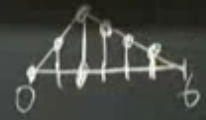
\includegraphics[height=2cm]{4_14.png}

Aslinda esitligin sag tarafinda delta (ve sabit) oldugu sartlarda
``sansliyiz'' cunku bu durumlarda ayriksal sonuc gercek sonucun tam ustunde
cikiyor. Bu sansliligin sebebi, aslinda, ustteki deltadan basamaga, oradan
rampaya, vs. gecmek icin kullandigimiz entegral yerine, ayriksalda toplama
kullaninca anlasiliyor, o gecis sirasinda da toplamlar ve entegraller
tam uyum halindeler, bu da dogal olarak diferansiyel denkleme yansiyor. 

Neyse, sayilari da yerine koyarak elle bulunabilecek bir sonuca
erisebiliriz.

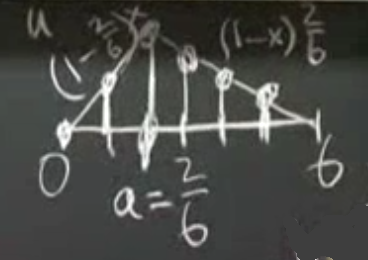
\includegraphics[height=2cm]{4_15.png}

Teori

\[ \int_{-\infty}^{\infty} \delta(x)g(x) dx = g(0)\]

Ispat

Parcali entegral yontemini uygularsak,

\[ \int u \ dv = uv - \int v \ du \]

\[ u = g(x), \ dv = \delta(x)dx \]

\[ \int_{-A}^{A} g(x)\delta(x) dx = g(x)u(x) \bigg]_{-A}^{A} -
\int_{-A}^{A} u(x) \frac{dg(x)}{dx}dx
\]

$-A$ ve $A$ entegral s�n�rlar� s�f�r� ortalayacak sekilde secilmis iki
degerdir, $A$ herhangi bir sayi olabilir. $u(x)$ $\delta(x)$ fonksiyonunun
entegrali olduguna gore $x=0$ oncesi sifir, sonrasi 1 olacak. O zaman
birinci k�s�m

\[ g(x)u(x) \bigg]_{-A}^{A} = g(x)u(x) \bigg]_{0}^{A} = g(A)\cdot 1 = g(A)\]

$x=0$ oncesi onemli degil cunku orada $u(x) = 0$. 

Ikinci kisim

\[ \int_0^A 1\cdot \frac{dg(x)}{dx}dx = g(A) - g(0) \]

Biraraya koyarsak

\[ g(A) - (g(A) - g(0)) = g(A) - g(A) + g(0) = g(0) \]

Ispat boylece tamamlaniyor.

Soru 1.2.2

$u''(x) = \delta(x)$, $u(-2) = 0$ ve $u(3) = 0$ problemini coz. Parcalar $u
= A(x+2)$ 
ve $u=B(x-3)$ $x=0$ noktasinda birlesiyor. $U = (u(-1), u(0), u(1), u(2))$  
vektorunun $KU=F=(0,1,0,0)$ problemini cozdugunu goster.

Cozum

Yukarida cozumun hangi formda olacagi $A$ ve $B$ uzerinden verilmis, burada
guzel bir numara var (alternatif cozumde bunu anlattik), fakat biz once
derste daha gosterilen yontem uzerinden cozumu kendimiz bulalim.

Ozel (particular) cozum nedir? 

\[ u(x) = -R(x) + C + Dx\]

Bildigimiz gibi $R(x)$ rampa fonksiyonu soyle:

\[ 
R(x) = \left\{ \begin{array}{ll}
0 & x \le 0 \\
x & x \ge 0 
\end{array} \right.
 \]

Simdi s�n�r sartlarini kullanarak $u(x)$ icinde yerine koyalim:

\[ u(-2) = -R(x) + C - 2D = 0 \]

\[ u(-2) = C - 2D = 0 \]

$x=-2$ yani sifirdan kucuk oldugu icin $-R(x)=0$ oldu ve onu formulden attik.

\[ u(3) = -3 + 3D + C = 0 \]

Burada $x=3$, o yuzden $-R(3) = -3$ kullanildi. Sonuc

\[ C = 2D \]

\[ 3 + 3D + 2D = 0 \]

\[ 5D - 3 = 0 \]

\[ D = \frac{3}{5} \]

O zaman

\[ C - 2(\frac{3}{5}) = 0 \]

\[ C = \frac{6}{5} \]

Sifirdan oncesi ve sonrasi icin (degisik $R(x)$ durumlarina gore)
fonksiyonu parcali bir sekilde yazarsak

\[ u(x) =
\left\{ \begin{array}{ll}
& \\
\frac{6}{5} + \frac{3}{5}x & x \le 0 \\
& \\
-x + \frac{6}{5} + \frac{3}{5}x = \frac{6}{5} - \frac{2}{5}x & x \ge 0 \\
& 
\end{array} \right.
 \]

Birinci kismi sadelestirirsek

\[ \frac{6}{5} + \frac{3}{5}x  = \frac{3}{5}(x + 2)  \]

Ikinci kismi sadelestirirsek

\[ \frac{6}{5} - \frac{2}{5}x =  -\frac{2}{5}(x - 3)\]

Problemin hazir verdigi forma, ve sonuca eristik.

\lstinputlisting[language=Python]{1.2.2.py}

\begin{lstlisting}[language=Python]
[[ 0.8  0.6  0.4  0.2]
 [ 0.6  1.2  0.8  0.4]
 [ 0.4  0.8  1.2  0.6]
 [ 0.2  0.4  0.6  0.8]]
\end{lstlisting}

Bir sonraki derste gorecegimiz gibi ustteki sonucun 2. kolonu aradigimiz
sonuc (cunku delta agirligi 2. hucre uzerinde). Bu kolondaki degerleri
teker teker $x=-1,0,1,2$ degerlerini $u(x)$'i hesaplayarak kontrol edelim.

\[ 6/5 + 3/5(-1) = 3/5 = 0.6 \]

\[ 6/5 + 3/5(0) = 6/5 = 1.2 \]

\[ 6/5 -2/5(1) = 4/5 = 0.8 \]

\[ 6/5 -2/5(2) = 2/5 = 0.4 \]

Sonuclar birebir uyuyor. 

Alternatif Cozum

Problemin cebirsel cozumu icin bir yontem daha var, hatta ders notlarindaki
1.2.2 cozumu bu yontemi kullaniyor. 

$u(x)$'in formunun lineer olacagini bildigimizden, ve bu formul icinde bir
rampa fonksiyonu olmasindan hareketle, cozumun iki lineer parca icerdigini
ve bu parcalarin 0 noktasinda birlestigini farzedebiliriz. Soyle iki
fonksiyon buluruz: $A(x+2)$ ve $B(x-3)$. Bu her iki fonksiyonun -2 ve +3
noktalarinda sifir olduguna dikkat, ki bu diferansiyel denklemin sinir
sartlari ile uyumlu.

Simdi alttaki numaralara bakalim, tek bir integral, ve tek bir turev alarak
cok daha basit cebirsel ifadelerle calisma imkani var. Iki tarafin
entegrali:

\[ -\int u''(x) = \int \delta(x) \]

\[ -[u'(x)]_L^R = 1 \]

R ve L sag (right) ve sol (left) ibareleri, delta fonksiyonunun yogunluk
yarattigi noktanin sagindaki ve solundaki herhangi birer nokta icin
kullaniliyor, delta fonksiyonunun entegralini alirken bu noktanin
``uzerinden gecersek'' sonuc her zaman 1 verecektir. O noktalarin tam
olarak ne oldugu onemli degil, cunku $x=0$ solunda ve solunda egim her
noktada ayni.

\[ u_R'(x) - u_L'(x) = -1 \]

Ustteki turevleri formlara uygulariz

\[ B - A = -1 \]

Iki parca $x=0$ noktasinda birlesiyor, o zaman

\[ A(0+2) = B(0-3) \]

\[ A = -\frac{3}{2}B \]

Birlestirince

\[ B - (-3/2 B ) = -1 \]

\[ B = -0.4 \]

\[ A = 0.6 \]

Soru 1.2.4

\lstinputlisting[language=Python]{1.2.4.py}

\begin{lstlisting}[language=Python]
[[ 1  0  0]
 [-1  1  0]
 [ 0 -1  1]]

[[ 1.  0.  0.]
 [ 1.  1.  0.]
 [ 1.  1.  1.]]
\end{lstlisting}

\verb!D_0! matrisini soruda istendigi sekilde yarattik. Bu matrisin null
uzayi, yani \verb!D_0 u = 0! denklemindeki $u$ sifir olmadigi icin, bu
matris tersine cevirilemez demektir, yani matris tekil (singular)
demektir. 

Soru 1.2.10

27. denklemden bahsediliyor, bu yanlis. Sorunun istedigini kodlamak daha
iyi: $\Delta_+$ icin \verb!DF! ve $\Delta_-$ yerine \verb!DB! kullanip,
carpimini alirsak,

\lstinputlisting[language=Python]{1.2.10.py}

Carpim

\begin{lstlisting}[language=Python]
[[-2  1  0]
 [ 1 -2  1]
 [ 0  1 -1]]
\end{lstlisting}

Bu matriste $u = 0$ sinir sartinin hangi satir ile temsil edildigi
soruluyor, yani $u(..) = 0$ sartinda '..' neresi? Bu sart icin sol taraftaki
kolonun atildigini hayal edelim, geriye kalanlar ust 1. satiri [-2 1]
uzerinden $u(0)=0$ sartini zorlar. Dogru cevap 1. satir.

Peki $u'(..) = 0$ sarti hangi satirla, yani hangi '..' degeriyle zorlanir?
En alt satir gibi duruyor, kontrol edelim, 

\[ \frac{u_4-u_3}{h} = 0\]

o zaman

\[ u_4 = u_3 \]

Matrisin en son satirini cebirsel sekilde yazalim

\[ \frac{u_4 - 2u_3 + u_2}{h} \]

$u_4 = u_3$ oldugu icin

\[ = \frac{u_3 - 2u_3 + u_2}{h} \]

\[ = \frac{-u_3 + u_2}{h} \]

Son ifade matrisin sonuncu satirini aynen tarif ediyor.

Soru 1.2.19

Cebirsel olarak bu denklemi cozmek icin onun sabit katsayili, 2. seviye
(homojen olmayan -sifira esit degil-) denklem oldugunu gormek yeterli. Once
ana denklemle baglantili homojen denklemi (sifira esitlenmis halini yani)
cozeriz.

\[ -u'' + u' = 0. \]

Bu denklemi cozmek icin karakteristik denklemini buluruz (bkz MIT OCW ODE
Ders 9). Bu denklem $-r^2 + r = 0$ olacaktir, kokleri  $0$ ve $1$, o zaman
homojen denklemin cozum yelpazesini $e^{0x}=1$ ve $e^{x}$ tanimlar. Genel
cozum demek ki

\[ \mathbf{s} + A + Be^x \]

olur, ki $A$ ve $B$ rasgele sabitlerdir, ve $\mathbf{s}$, $-u''+u'=1$ denkleminin
ozel (particular) bir cozumudur. $u(x)=x$'in bu ozel cozum oldugunu bulmak
zor degildir, o zaman cozumun tamami

\[ u(x) = x + A + Be^x \]

olacaktir. 

\[ u(0) = A + B = 0 \]

\[ A = -B \]

\[ u(1) = 1 + -B + Be^1 = 0\]

\[ B = \frac{1}{1-e} \]

\[ A = \frac{-1}{1-e} \]

Denklemin tam cozumu

\[ u(x) = x - \frac{1}{1-e} + \frac{1}{1-e}e^x \]

\lstinputlisting[language=Python]{1.2.19.py}

Sonuc (numerik cozum)

\begin{lstlisting}[language=Python]
ortalanmis [ 0.07135546  0.11412325  0.12195055  0.0870728 ]

ileri farklilik [ 0.07956826  0.123533    0.12793827  0.08838856]
\end{lstlisting}

Bu cozumlerden ortalanmis olanin daha iyi oldugunu gorebiliriz. 

Soru 1.2.21

$u(h) = u(0) + hu'(0) + \frac{1}{2}h^2u''(0)+..$ acilimini ve ``sifir egim
kosulu'' yani $u'(0) = 0$ olarak belirtilen sinir sartini ve $-u'' = f(x)$
ifadesini kullanarak $u_0 - u_1 = \frac{1}{2}h^2f(0)$ seklinde ust sinir
sartini turet. $\frac{1}{2}$ faktoru $O(h)$ hatasindan kurtulmamiza
yarayacak. 

Oncelikle turetmemiz istenen seyin 2. Ders Problem 1.2 A'da kullanilan
ifade ile ayni oldugunu gorelim. O problemde $u_0 - u_1 =
\frac{1}{2}h^2f(0)$ ifadesine farkli bir yonden erismistik, orada ortalama
farklilik teknigini kullanmistik. Burada Taylor acilimini kullaniyoruz, ve
ayni noktaya geliyoruz! 

$u(0)$ noktasindayiz, ve ileri dogru $h$ adimi atiyoruz, bu adimi Taylor
acilimi ile nasil gosteririz?

\[ u(h) = u(0) + h \cdot u'(0) + \frac{1}{2}h^2u''(0) + ... \]

Degil mi? Simdi, elimizde diferansiyel denklemin tanimindan gelen bazi
tanimlari kullanarak ustteki denklemi degistirelim. $-u''(x) = f(x)$ ise,
$u''(0) = -f(0)$ demektir. Ayrica $u'(0) = 0$ ise $h \cdot u'(0)$
denklemden atilabilir. Noktadan sonrasini biz atiyoruz, yaklasiksal olarak
temsil ettigimiz icin, o zaman

\[ u(h) = u(0) - \frac{1}{2}h^2f(0) \]

\[ u_1 - u_0 = -\frac{1}{2}h^2f(0)\]

\[ u_0 - u_1 = \frac{1}{2}h^2f(0) \]

Ve Cozulmus Problem 1.2 A'daki tanimin aynisina eristik. 

Problem 1.4.5

$-u''= \delta(x-a)$ denkleminin serbest-serbest sartlari, yani $u'(0) = 0$
ve $u'(1) = 0$ uzerinden cozumu {\em olamayacagini} goster, bu durumda $C$
ve $D$ sabitleri bulunamayacak. 

Cozum

Tam cozum neydi? 

\[ u(x) = R(x-a) + Cx + D \]

Eldeki sartlar sadece $u'(x)$ icin olduguna gore ustteki denklemin turevini
alalim, ve 0 ve 1 degerlerini yerine koyarak ele gecen sonuca bakalim. 

\[ u'(0) = 0 + C = 0 \]

Rampa fonksiyonunun turevi basamak fonksiyonu, fakat o noktada daha basamak
baslamamis (yani sifir seviyesinde). Aslinda soruda $a > 0$ bilgisini
verseler iyi olurdu, her neyse, bu sebeple ilk terim 0. $Cx$'den geriye $C$
kalir, $D$ yokolur.

\[ C = 0 \]

Diger kosulla

\[ u'(1) = -1 + C + 0 = 0 \]

Bu noktada basamak baslamis, cunku $a$ noktasi ilerisindeyiz, 
basamak fonksiyonu 1 degerinde, negatifi alindigi icin sonuc -1. Devam
edersek: 

\[ C = 1 \]

Bu bir absurtluk ortaya cikarti, $C$'nin hem 0 hem 1 olmasi mumkun
degildir. Demek ki serbest-serbest probleminin cozumu yoktur. 

\end{document}

